\documentclass[12pt, spanish]{article}
\usepackage[spanish]{babel}
\selectlanguage{spanish}
%\usepackage{natbib}
\usepackage{url}
\usepackage[utf8x]{inputenc}
\usepackage{graphicx}
\graphicspath{{images/}}
\usepackage{parskip}
\usepackage{fancyhdr}
\usepackage{vmargin}
\usepackage{multirow}
\usepackage{float}
\usepackage{chngpage}

\usepackage{amsfonts}

\usepackage{subcaption}

\usepackage{hyperref}
\usepackage[
    type={CC},
    modifier={by-nc-sa},
    version={4.0},
]{doclicense}

\hypersetup{
    colorlinks=true,
    linkcolor=blue,
    filecolor=magenta,
    urlcolor=cyan,
}

% para codigo
\usepackage{listings}
\usepackage{xcolor}



%% configuración de listings

\definecolor{listing-background}{HTML}{F7F7F7}
\definecolor{listing-rule}{HTML}{B3B2B3}
\definecolor{listing-numbers}{HTML}{B3B2B3}
\definecolor{listing-text-color}{HTML}{000000}
\definecolor{listing-keyword}{HTML}{435489}
\definecolor{listing-identifier}{HTML}{435489}
\definecolor{listing-string}{HTML}{00999A}
\definecolor{listing-comment}{HTML}{8E8E8E}
\definecolor{listing-javadoc-comment}{HTML}{006CA9}

\lstdefinestyle{eisvogel_listing_style}{
  language         = python,
%$if(listings-disable-line-numbers)$
%  xleftmargin      = 0.6em,
%  framexleftmargin = 0.4em,
%$else$
  numbers          = left,
  xleftmargin      = 0em,
 framexleftmargin = 0em,
%$endif$
  backgroundcolor  = \color{listing-background},
  basicstyle       = \color{listing-text-color}\small\ttfamily{}\linespread{1.15}, % print whole listing small
  breaklines       = true,
  frame            = single,
  framesep         = 0.19em,
  rulecolor        = \color{listing-rule},
  frameround       = ffff,
  tabsize          = 4,
  numberstyle      = \color{listing-numbers},
  aboveskip        = 1.0em,
  belowskip        = 0.1em,
  abovecaptionskip = 0em,
  belowcaptionskip = 1.0em,
  keywordstyle     = \color{listing-keyword}\bfseries,
  classoffset      = 0,
  sensitive        = true,
  identifierstyle  = \color{listing-identifier},
  commentstyle     = \color{listing-comment},
  morecomment      = [s][\color{listing-javadoc-comment}]{/**}{*/},
  stringstyle      = \color{listing-string},
  showstringspaces = false,
  escapeinside     = {/*@}{@*/}, % Allow LaTeX inside these special comments
  literate         =
  {á}{{\'a}}1 {é}{{\'e}}1 {í}{{\'i}}1 {ó}{{\'o}}1 {ú}{{\'u}}1
  {Á}{{\'A}}1 {É}{{\'E}}1 {Í}{{\'I}}1 {Ó}{{\'O}}1 {Ú}{{\'U}}1
  {à}{{\`a}}1 {è}{{\'e}}1 {ì}{{\`i}}1 {ò}{{\`o}}1 {ù}{{\`u}}1
  {À}{{\`A}}1 {È}{{\'E}}1 {Ì}{{\`I}}1 {Ò}{{\`O}}1 {Ù}{{\`U}}1
  {ä}{{\"a}}1 {ë}{{\"e}}1 {ï}{{\"i}}1 {ö}{{\"o}}1 {ü}{{\"u}}1
  {Ä}{{\"A}}1 {Ë}{{\"E}}1 {Ï}{{\"I}}1 {Ö}{{\"O}}1 {Ü}{{\"U}}1
  {â}{{\^a}}1 {ê}{{\^e}}1 {î}{{\^i}}1 {ô}{{\^o}}1 {û}{{\^u}}1
  {Â}{{\^A}}1 {Ê}{{\^E}}1 {Î}{{\^I}}1 {Ô}{{\^O}}1 {Û}{{\^U}}1
  {œ}{{\oe}}1 {Œ}{{\OE}}1 {æ}{{\ae}}1 {Æ}{{\AE}}1 {ß}{{\ss}}1
  {ç}{{\c c}}1 {Ç}{{\c C}}1 {ø}{{\o}}1 {å}{{\r a}}1 {Å}{{\r A}}1
  {€}{{\EUR}}1 {£}{{\pounds}}1 {«}{{\guillemotleft}}1
  {»}{{\guillemotright}}1 {ñ}{{\~n}}1 {Ñ}{{\~N}}1 {¿}{{?`}}1
  {…}{{\ldots}}1 {≥}{{>=}}1 {≤}{{<=}}1 {„}{{\glqq}}1 {“}{{\grqq}}1
  {”}{{''}}1
}
\lstset{style=eisvogel_listing_style}


\usepackage[default]{sourcesanspro}

\setmarginsrb{2 cm}{1 cm}{2 cm}{2 cm}{1 cm}{1.5 cm}{1 cm}{1.5 cm}

\title{Práctica 3:\\
Detección de puntos relevantes y creación de panoramas.\hspace{0.05cm} }
\author{Antonio David Villegas Yeguas}
\date{\today}

\renewcommand*\contentsname{hola}

\makeatletter
\let\thetitle\@title
\let\theauthor\@author
\let\thedate\@date
\makeatother

\pagestyle{fancy}
\fancyhf{}
\rhead{\theauthor}
\lhead{\thetitle}
\cfoot{\thepage}

\begin{document}

%%%%%%%%%%%%%%%%%%%%%%%%%%%%%%%%%%%%%%%%%%%%%%%%%%%%%%%%%%%%%%%%%%%%%%%%%%%%%%%%%%%%%%%%%

\begin{titlepage}
    \centering
    \vspace*{0.3 cm}
    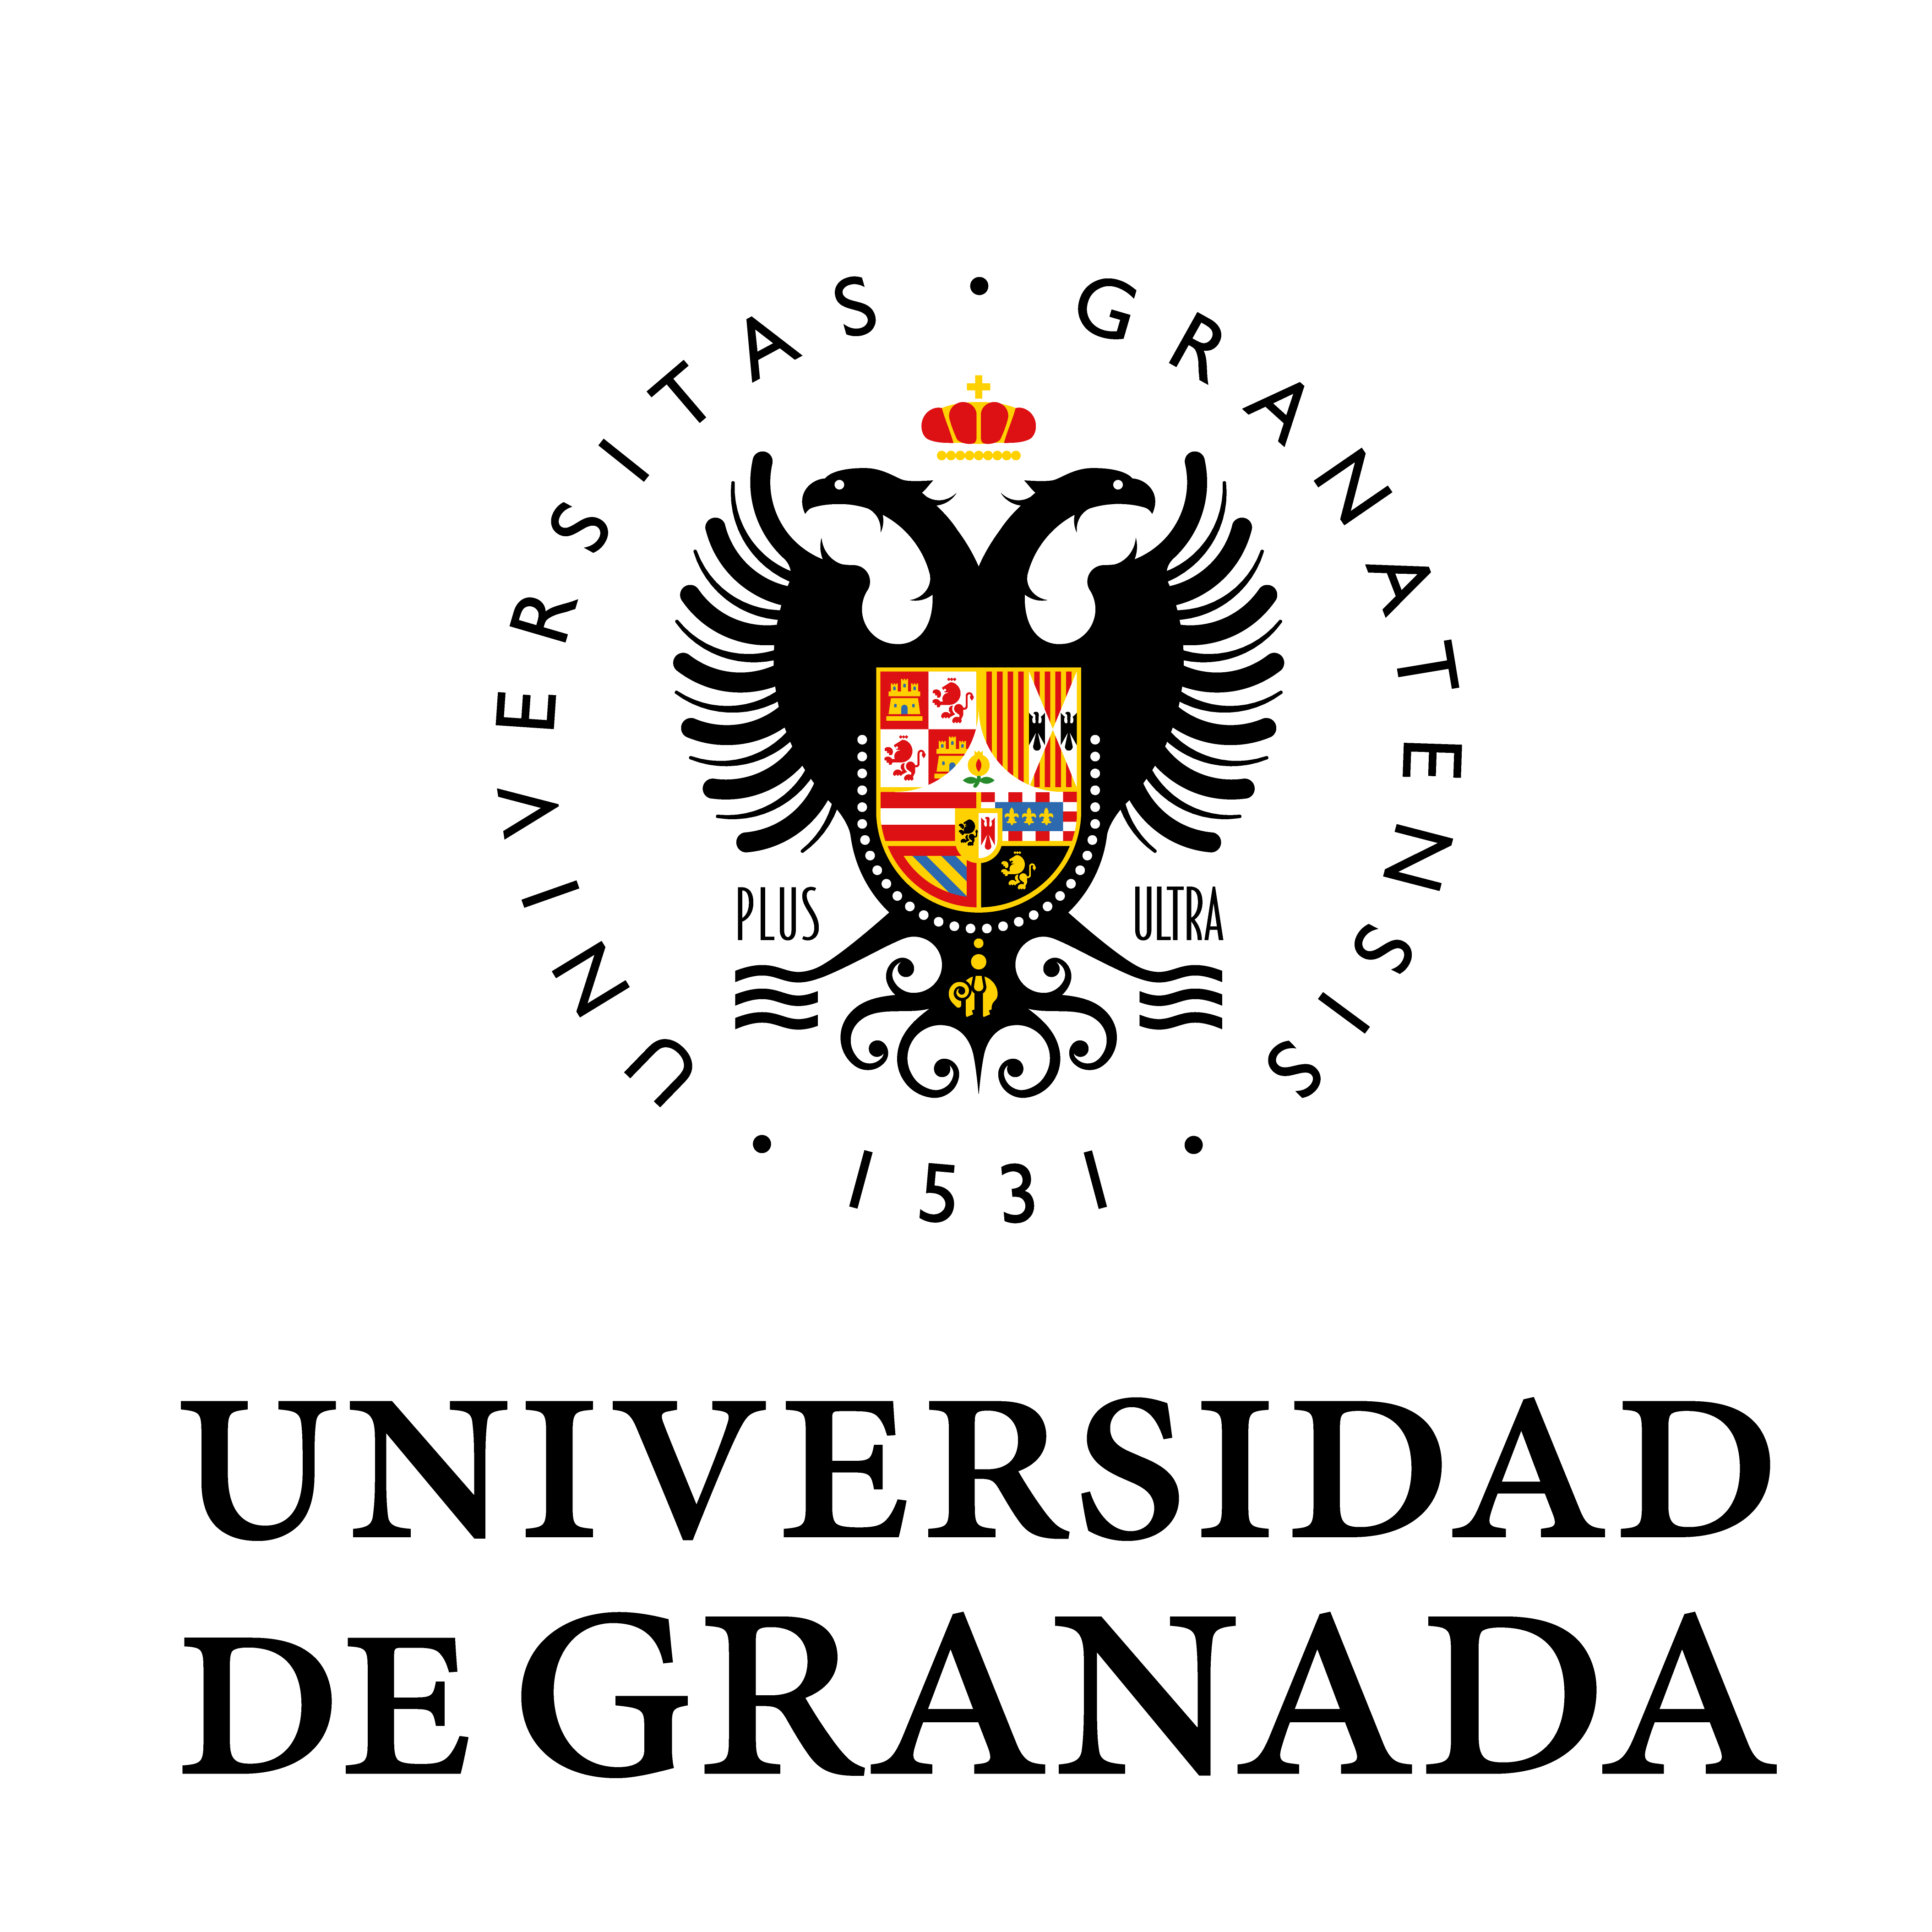
\includegraphics[scale = 0.50]{ugr.png}\\[0.7 cm]
    %\textsc{\LARGE Universidad de Granada}\\[2.0 cm]
    \textsc{\large 4º CSI 2020/21 - Grupo 2}\\[0.5 cm]
    \textsc{\large Grado en Ingeniería Informática}\\[0.5 cm]
    \rule{\linewidth}{0.2 mm} \\[0.2 cm]
    { \huge \bfseries \thetitle}\\
    \rule{\linewidth}{0.2 mm} \\[1 cm]

    \begin{minipage}{0.4\textwidth}
        \begin{flushleft} \large
            \emph{Autor:}\\
            \theauthor\\
			 \emph{DNI:}\\
            77021623-M
            \end{flushleft}
            \end{minipage}~
            \begin{minipage}{0.4\textwidth}
            \begin{flushright} \large
            \emph{Asignatura: \\
            Visión por Computador}   \\
            \emph{Correo:}\\
            advy99@correo.ugr.es
        \end{flushright}
    \end{minipage}\\[0.5cm]

    {\large \thedate}\\[0.5cm]
    %{\url{https://github.com/advy99/VC/}}
    {\doclicenseThis}

    \vfill

\end{titlepage}

%%%%%%%%%%%%%%%%%%%%%%%%%%%%%%%%%%%%%%%%%%%%%%%%%%%%%%%%%%%%%%%%%%%%%%%%%%%%%%%%%%%%%%%%%

\tableofcontents
\pagebreak

%%%%%%%%%%%%%%%%%%%%%%%%%%%%%%%%%%%%%%%%%%%%%%%%%%%%%%%%%%%%%%%%%%%%%%%%%%%%%%%%%%%%%%%%%


\section*{Introducción}

Tras haber realizado una introducción a OpenCV en la práctica cero, trabajado con filtros sobre imágenes en la práctica uno, y clasificado imágenes utilizando redes neuronales convolucionales en la práctica dos, en esta práctica trabajaremos con la información de la geometría de las imágenes, en concreto con la detección de puntos de interes, su detección y uso para realizar otras operaciones como la detección de un objeto o zona de una imagen dentro de otra, lo que también nos permitirá por último crear panoramas de imágenes.

Trabajaremos con puntos Harris, descriptores de puntos con AKAZE, y por último creación de panoramas utilizando los puntos de interes y descriptores AKAZE.

\section{Detección de punto Harris}

Este apartado trata sobre la detección de puntos de interes utilizando el algoritmo de detección de esquinas Harris, que se trata de, utilizando una pirámide gaussiana de la imagen sobre la que obtener los puntos de interes de cara a trabajar con varias escalas y una pirámide con las derivadas de cara a obtener el gradiente, calcular los puntos de interes usando el criterio de Harris, aplicar una supresión de no máximos de cara a quedarse con los más prometedores y con estos calcular su orientación utilizando su gradiente\cite{harris}.

En mayor detalle, para cada escala (nivel de la pirámide construida), realizaremos:

\begin{enumerate}
	\item Detección de puntos de interes: Utilizando la función de OpenCV \texttt{cornerEigenValsAndVecs}\cite{cornerCV} obtendremos los valores singulares, para despues aplicarles el criterio Harris: $\frac{\lambda_{1} \lambda_{2}}{\lambda_{1} + \lambda_{2}}$.
	\item Aplicar el umbral Harris: Eliminar los valores por debajo de este umbral.
	\item Supresión de no máximos: Dado un tamaño de ventana, recorreremos la imagen actual con ese tamaño de ventana, obteniendo el valor máximo de la ventana actual, y si el centro de la ventana (pixel actual) es el máximo, almacenaremos ese valor en el resultado, si no, lo descartaremos.
	\item Estimación de la escala de los puntos en píxeles: Como nos dice en el guión, haremos una estimación de la escala de forma que sea igual a $2^{nivel\_piramide - 1} \cdot tam\_bloque$.
	\item Calculo de la orientación de los puntos: Utilizando el gradiente de los puntos considerados de interes, calcularemos la norma de dichos puntos y con eso su orientación. Como nos dice el guión, en este apartado utilizaremos el gradiente de las imágenes aplicandole un alisamiento con $\sigma = 4.5$.
	\item Calculo del KeyPoint de OpenCV utilizando el método \texttt{KeyPoint} y los valores calculados.
\end{enumerate}

Y con esto ya tendremos los puntos de interes. Además de estos puntos, la función implementada devolverá los puntos corregidos, que son calculados de la siguiente forma:

\begin{enumerate}
	\item Concatenar los valores de X e Y de los puntos en un vector fila, de cara a poder utilizarlos en el siguiente punto.
	\item Utilizar el método \texttt{cornerSubPix} como nos dice el guión para obtener los puntos corregidos, usando como criterio de parada quince iteraciones o un epsilon menos a $0.01$. Se han escogido estos valores ya que han funcionado bastante bien de forma empírica.
	\item Redondeo y adaptación de los ejes de los puntos obtenidos por la función \texttt{cornerSubPix}.
\end{enumerate}


Como vemos, en este apartado tenemos bastantes parámetros con los que trabajar:

\begin{enumerate}
	\item Tamaño del bloque: Fijado a cinco, como nos decía el guión, podía ser desde 3x3 a 7x7, en mi caso el tamaño cinco se ha comportado bastante bien de forma empírica, y por eso lo he escogido.
	\item Tamaño de la ventana: En este caso se nos daba entre utilizar tamaños 3x3, 5x5 y 7x7. Al utilizar tamaños más pequeños se obtenian muchos más puntos, ya que tendríamos un mayor número de ventanas, pero se obtenian demasiados puntos para el umbral utilizado (que comentaré más adelante), por este motivo he utilizado el tamaño 7x7.
	\item Número de escalas: Como nos decía el guión, tres escalas.
	\item Sigma de la pirámide Gaussiana: En este caso, como nos comentaba el guión, he utilizado $\sigma = 4.5$.
	\item Umbral del criterio Harris: Como nos decía la bibliografía\cite{harris}, he utilizado un umbral $t = 10.0$, en los resultados de este apartado pondré un ejemplo de utilizar un umbrál distinto.
	\item Tamaño del kernel para calcular las derivadas: En este caso también se nos recomendaban los valores de ksize de tres o cinco, y en mi caso he optado por el valor tres ya que se comportaba de forma correcta.
\end{enumerate}

Tras describir la función con la que obtenemos los puntos Harris a las distintas escalas, para visualizarlos simplemente se ha usado una lista con todos los puntos (de todas las escalas), y se ha utilizado el método \texttt{drawKeypoints} para dibujarlos sobre la imagen, utilizando la opción\\  \texttt{DRAW\_MATCHES\_FLAGS\_DRAW\_RICH\_KEYPOINTS} de forma que dibujará los puntos acorde a la escala, y con su orientación.

Otro detalle a tener en cuenta es que aunque se ha utilizado la imagen en blanco y negro para obtener los puntos (como nos recomendaba el guión y nos obliga OpenCV), se han mostrado sobre la imagen a color para quela distinción de los puntos sobre la imagen sea más llamativa. Se ha obtenido el siguiente resultado:


\begin{figure}[H]
  \centering
      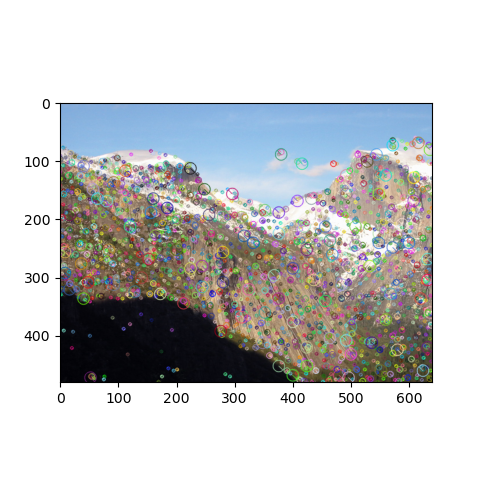
\includegraphics[width=\textwidth]{p_harris_h_10.png}
 		\caption{Puntos Harris sobre la imágen Yosemite1.}
\end{figure}

\begin{figure}[H]
  \centering
      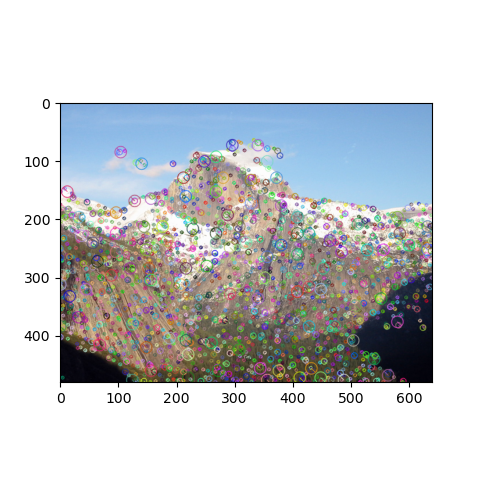
\includegraphics[width=\textwidth]{p_harris_h_10_y2.png}
 		\caption{Puntos Harris sobre la imágen Yosemite2.}
\end{figure}

Como vemos los resultados son bastante buenos, y como se nos pedía, hemos calculado unos 2000 puntos en cada imágen, distribuidos de la siguiente forma.

Para la imagen Yosemite1:

\begin{lstlisting}
La escala  0  tiene  1478  puntos
La escala  1  tiene  375  puntos
La escala  2  tiene  109  puntos
\end{lstlisting}

Para la imagen Yosemite2:

\begin{lstlisting}
La escala  0  tiene  1506  puntos
La escala  1  tiene  392  puntos
La escala  2  tiene  114  puntos
\end{lstlisting}

Tal y como nos pedía el guión, alrededor de un 70\% de los puntos en el nivel más grande, un 25\% en el siguiente nivel, y por último el 5\% restante en el nivel más bajo.


Como hemos visto, la mayoría de parámetros son parámetros que ya hemos visto y estudiado en otras prácticas (en especial la primera), sin embargo, aquí aparece un nuevo parámetro, el umbral Harris, que de cara a estudiar su importancia, he repetido la prueba de Yosemite1 pero utilizando un umbral de 300 en lugar de 10:

\begin{figure}[H]
  \centering
      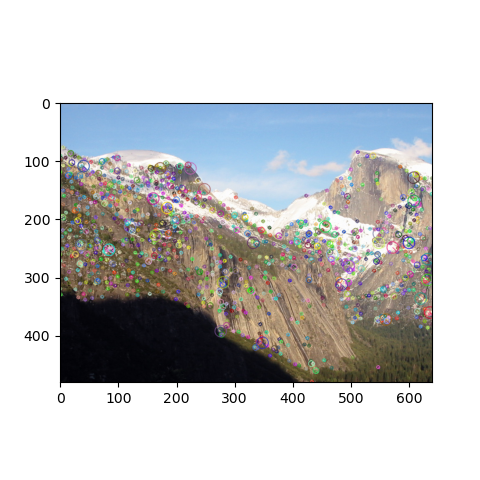
\includegraphics[width=\textwidth]{p_harris_h_300.png}
 		\caption{Puntos Harris sobre la imágen Yosemite1 con umbral Harris de 300.}
\end{figure}

Con el que obtenemos el siguiente número de puntos:

\begin{lstlisting}
La escala  0  tiene  915  puntos
La escala  1  tiene  155  puntos
La escala  2  tiene  31  puntos
\end{lstlisting}

Como era de esperar, se eliminan muchos de los puntos de interes obtenidos, aunque los parámetros son los mismos a excepción del umbral, por lo que este parámetro nos puede ayudar a ajustar el número de puntos a obtener manteniendo la forma de calcular los distintos puntos, al mantener los tamaños de bloque, ksize, entre otros.



Por último para este ejercicio compararemos los puntos originales con los puntos corregidos.

Para realizar esta comparación se han escogido tres puntos al azar donde su posición original es distinta a la posición corregida, y se han dibujado como círculos de radio 2 píxeles en la imagen, para despues mostrar una ventana de 9x9 como nos piden, de forma que se distinga la posición de los puntos. El resultado es el siguiente, con el punto original en azul y en rojo el corregido:

\begin{figure}[H]
  \centering
      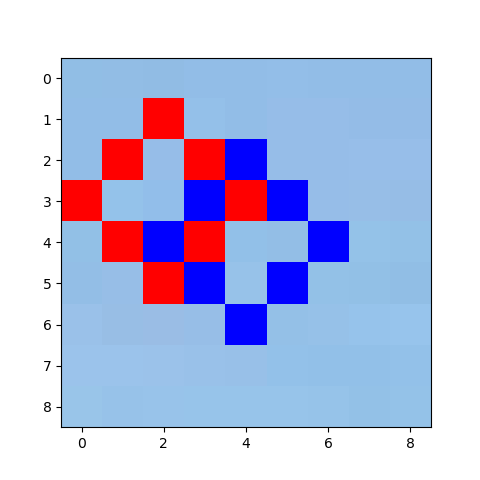
\includegraphics[width=\textwidth]{cmp_p1.png}
 		\caption{Primer punto corregido escogido al azar.}
\end{figure}

\begin{figure}[H]
  \centering
      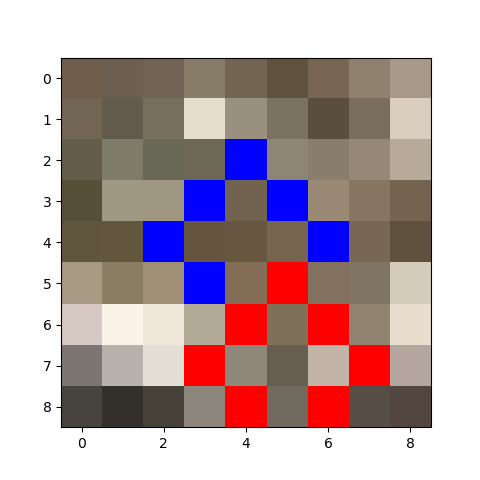
\includegraphics[width=\textwidth]{cmp_p2.png}
 		\caption{Segundo punto corregido escogido al azar.}
\end{figure}

\begin{figure}[H]
  \centering
      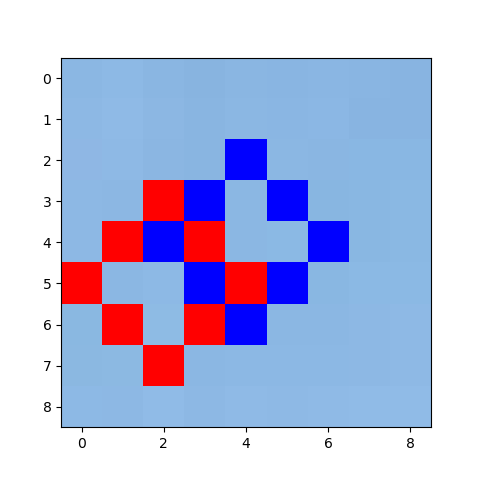
\includegraphics[width=\textwidth]{cmp_p3.png}
 		\caption{Tercer punto corregido escogido al azar.}
\end{figure}


Se puede observar como se modifican ligeramente las posiciones de los puntos, y a excepción del tercer punto donde todo el fondo es azul claro, en los otros dos casos se mmueve a una zona donde hay una mayor variación entre píxeles.


\section{Descriptores AKAZE y correspondencias entre dos imágenes}

En este apartado nos centraremos en dectecar los puntos de interes así como sus descriptores utilizando AKAZE\cite{akaze}, la versión acelerada de KAZE\cite{kaze}.

Para este ejercicio se ha hecho uso del método \texttt{AKAZE\_create} de OpenCV para crear un objeto de la clase AKAZE, con el que calcularemos los puntos clave y los descriptores de la imagen.

Aunque se han utilizado los parámetros por defecto, he añadido el parámetro de umbral de cara a crear el detector AKAZE. Este umbral será el umbral será el umbral para aceptar un punto y usaremos el valor por defecto en OpenCV, $0.1$.

Para obtener los descriptores y los puntos clave, simplemente se llamará a la función \texttt{detectAndCompute} de la instancia creada de AKAZE.


Una vez tenemos los descriptores y puntos de dos imágenes necesitamos encontrar las coincidencias entre estos dos. Para esto usaremos dos métodos, ambos utilizando un objeto de la clase \texttt{BFMatcher} de OpenCV:

\begin{enumerate}
	\item Fuerza bruta con validación cruzada: Utilizando el método \texttt{match}, pasando como argumento los descriptores de ambas imágenes, obtendremos las coincidencias utilizando un algoritmo de fuerza bruta. Para utilizar validación cruzada será necesario establecer el parámetro \texttt{crossCheck} a verdadero en la creación del objeto BFMatcher.
	\item Clasificador 2NN aplicando el criterio de Lowe: Al igual que el anterior, pero en lugar de utilizar el método \texttt{match} utilizaremos el método \texttt{knnMatch} con $k = 2$, y al resultado le aplicaremos el criterio de Lowe. Este criterio se basa en eliminar todas las coincidencias donde el radio de la distancia entre los puntos es mayor que el $0.8$, consiguiendo eliminar alrededor de un 90\% de falsos positivos, y eliminando únicamente alrededor de un 5\% de coincidencias reales\cite{lowe}.
\end{enumerate}


Una vez tenemos tanto los puntos clave como las coincidencias, dibujamos los resultados utilizando el método de OpenCV \texttt{drawMatches}. Como nos dice el guión, escogeremos cien coincidencias aleatorias y solo dibujaremos esas, de cara a poder distinguir con claridad los resultados:

\begin{figure}[H]
  \centering
      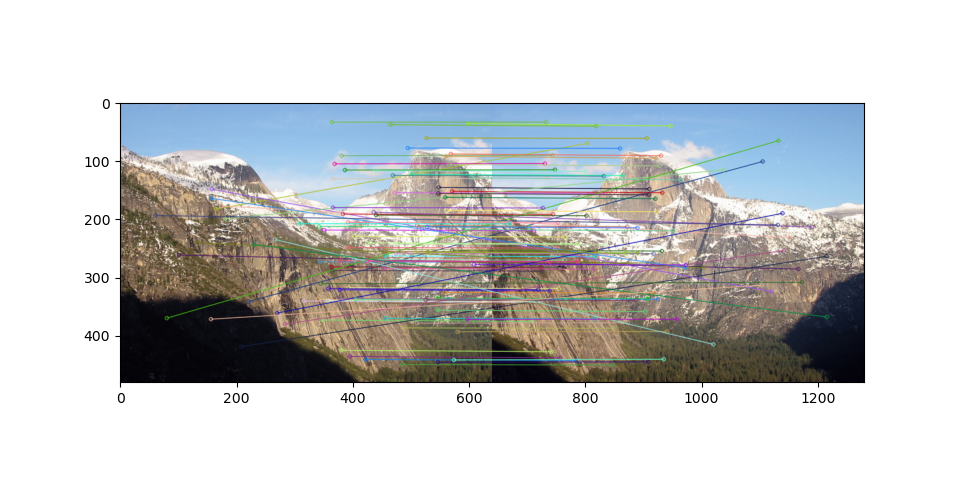
\includegraphics[width=\textwidth]{correspondencias_fuerza_bruta.png}
 		\caption{Correspondencias entre Yosemite1 y Yosemite2 utilizando fuerza bruta con validación cruzada.}
\end{figure}

\begin{figure}[H]
  \centering
      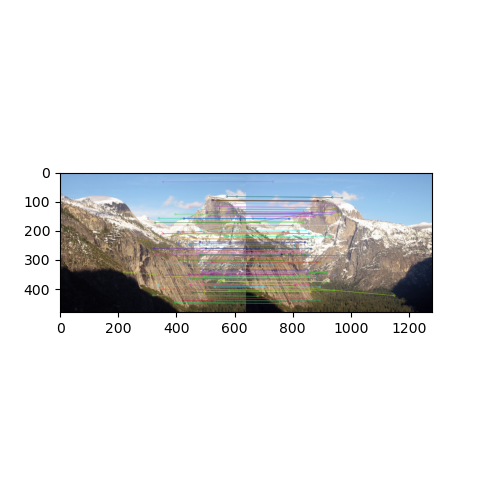
\includegraphics[width=\textwidth]{correspondencias_lowe_2nn.png}
 		\caption{Correspondencias entre Yosemite1 y Yosemite2 utilizando 2NN y aplicando el criterio de Lowe.}
\end{figure}


Como vemos, el método de fuerza bruta con validación cruzada queda bastante atrás con respecto al método de 2NN con el criterio de Lowe, ya que como podemos observar se consigue un número de errores considerablemente menor.

En especial vemos como la mayoría de fallos utilizando fuerza bruta se producen entre puntos con gran distancia, por lo que en el caso en el que utilizamos el criterio de Lowe observamos que no se producen tantos errores. Aun así si se siguen produciendo errores en el caso de 2NN con el criterio de Lowe, aunque se tratan más bien de casos excepcionales que en lo común, al contrario que en el primer caso.

Otra de las tendencias que podemos observar es que los errores que se producen en las mismas zonas de la primera imagen, llevan a puntos (en este caso erroneos) de las mismas zonas en la segunda imagen, como por ejemplo, los puntos de la zona sombreada más a la izquierda de la primera imagen suelen coincidir con la zona central superior de la segunda imagen, ya que los interpreta como zonas similares, aunque en este caso sea erroneo.


\newpage

\section{Mosaico de imágenes}

Tras haber trabajado la detección de puntos de interes, la extracción de descriptores y usado ambos para buscar correspondencias entre dos imágenes el siguiente paso es utilizar dichas correspondencias para crear un panorama con tres imágenes.

En este caso, además de utilizar los puntos de interes y descriptores de una imagen también utilizaremos las homografías. Una homografía se trata de una relación entre dos imágenes que comparten el mismo plano, es decir, si dos imágenes son similares o iguales, pero tomadas desde distintas posiciones, ambas imágenes estarán relacionadas por una homografía, de forma que si aplicamos la homografía a una de estas obtendremos la otra.

Gracias al uso de homografías conseguiremos crear mosaicos entre dos imágenes A y B siguiendo los siguientes pasos:

\begin{enumerate}
	\item Calculamos los puntos clave y los descriptores de las imágenes A y B.
	\item Buscamos las coincidencias entre los puntos clave.
	\item Calculamos la homografía que relaciona ambas imágenes utilizando el método \texttt{findHomography} de OpenCV.
	\item Fusionamos ambas imágenes utilizando el método \texttt{warpPerspective} de OpenCV y la homografía calculada en el paso anterior. Como nos sugiere el guión de la práctica, usaré como borde \texttt{BORDER\_TRANSPARENT} de cara a que no se perciba el borde en el resultado.
\end{enumerate}

De esta forma obtendremos el mosaico entre dos imágenes A y B.

Para conseguir un mosaico con tres imágenes lo que haremos será situar la imagen central en el lienzo del resultado, calcularemos el mosaico de la imagen central y la de la izquierda, y tras esto el mosaico de la imagen centra y la imagen de la derecha.

Algunos detalles de implementación es que el lienzo del resultado, como no sabemos su tamaño a priori, será del mayor tamaño posible, la suma de todos los tamaños de las imágenes. Como al calcular las homografías tanto de la izquierda como de la derecha conocemos la posición final de estas imágenes, luego recortaré el resultado para eliminar las zonas negras sin información del mosaico.

Otro detalle es que inicialmente la imagen central se colocará en el centro del lienzo de resultado ya que no sabemos cuanto ocupará el resultado y como vimos en teoría, al realizar los mosaicos habrá cierta deformación en las imágenes, y la central no se verá afectada, por lo que es la primera imagen a añadir.

Debido a la similitud con el siguiente ejercicio, se ha implementado directamente el siguiente ejercicio ya que es una generalización de este, y los detalles de dicha generalización los explicaré en el siguiente apartado.

El último detalle de implementación es que se ha utilizado el algoritmo RANSAC con un error máximo de 5 reproyecciones, ya que el método por defecto, minimos cuadrados, no nos ofrece unos buenos resultados.


El resultado es el siguiente:


\begin{figure}[H]
  \centering
      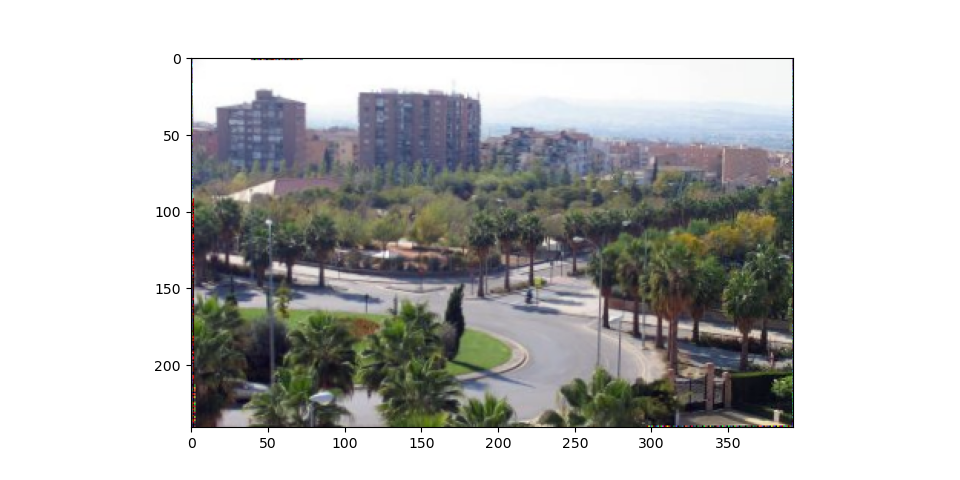
\includegraphics[width=\textwidth]{mosaico_tres_imagenes.png}
 		\caption{Mosaico de tres imágenes de las vistas de la ETSIIT.}
\end{figure}

Vemos como el resultado es bastante bueno, y apenas se nota el cambio entre imágenes.


\section{Mosaico con un número indefinido de imágenes}

Tras finalizar el apartado anterior, este apartado se trata simplemente de generalizar la creación del mosaico.

Al igual que en el apartado anterior, posicionaremos la imagen central en el centro del resultado, pero en lugar de buscar una homografia con la izquierda y añadirla, recorreremos todas las imágenes a la izquierda, buscando los puntos de interes y descriptores de una imagen y la anterior, buscando su homografía y aplicando el \texttt{warpPerspective} para obtener la solución hasta llegar al inicio de las imágenes, y tras esto realizaremos la misma operación pero desde el centro hasta el final de la lista de imágenes.

Como detalle importante, tendremos la homografía original (posición de la imagen central) almacenada, de forma que para calcular las homografías de las imágenes de la izquierda partiremos de esta, e iremos apilandolo las homografías para calcular la posición de una imagen con respecto a la posición de donde hemos colocado la anterior, no la central.

Una vez acabamos con las imágenes de la izquierda, como pasamos otra vez a calcular desde el centro a la derecha, volveremos a comenzar con la homografia de la imagen central y apilando las homografías calculadas a la derecha.

Al igual que en el apartado anterior, al apilar las homografías, podemos saber el tamaño real del resultado, ya que está almacenado en estas homografías, añadiendo ciertos márgenes a la derecha, ya que la homografía almacena el lugar donde se comienza a dibujar la imagen, no donde acaba, por lo que hay que añadir el espacio de la última imagen a la derecha y un margen para la deformación que hay podido sufrir.

\begin{figure}[H]
  \centering
      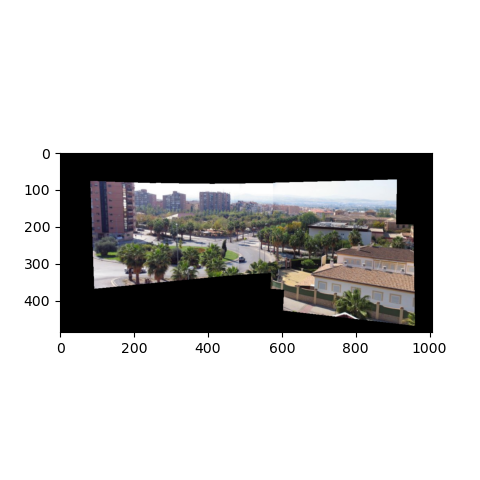
\includegraphics[width=\textwidth]{mosaico_etsiit.png}
 		\caption{Mosaico de todas las imágenes de las vistas de la ETSIIT.}
\end{figure}

Vemos como de nuevo el resultado es bastante bueno, siendo el esperado, por lo que podemos comprobar que este método es un método que nos permite construir panoramas con gran calidad, y en poco tiempo.


\newpage

Como prueba de consistencia del algoritmo implementado he realizado la prueba con dos imágenes, obteniendo un buen resultado y comprobando que el algoritmo realmente es dinámico y se puede utilizar tantas imágenes como se deseen:


\begin{figure}[H]
  \centering
      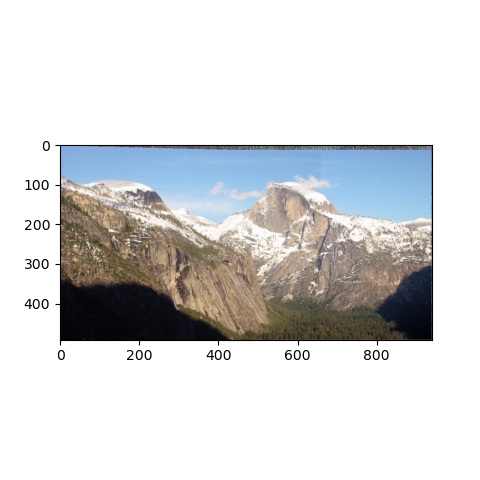
\includegraphics[width=\textwidth]{mosaico_dos_imagenes.png}
 		\caption{Mosaico de Yosemite1 y Yosemite2.}
\end{figure}


\newpage


\section{Bonus: Implementación propia de RANSAC}

De apartado opcional se nos pide implementar el algoritmo RANSAC para el cálculo de la homografía dados los puntos de interes de dos imágenes. Para desarrollar este apartado me he basado en el trabajo de Harshal Patil y de Prof.S.S.Deshmukh\cite{ransac} de cara a realizar una implementación en tiempo real del algoritmo RANSAC.

Esta implementación se basa en 7 pasos:

\begin{enumerate}
	\item Escoger cuatro puntos aleatorios de la lista de entre los puntos coincidentes.
	\item Obtener la homografía que relaciona esos cuatro puntos.
	\item Aplicar la homografía obtenida a toda la lista de puntos de correspondencias.
	\item Buscar la distancia entre los puntos usando la homografía.
	\item Si la distancia es menor que un umbral dado por el usuario, es un punto inlier.
	\item Volver a repetir el bucle hasta el máximo de iteraciones o tenemos suficientes puntos inlier.
	\item La homografía que más puntos inlier consiga es la mejor homografía y por tanto el resultado.
\end{enumerate}


Este algoritmo solo necesitará de entrada ambas listas de puntos, y el umbral a utilizar. Tras esto, he creado una función exactamente igual a la función del apartado 4, pero utilizando este método en lugar del método \texttt{findHomography} de OpenCV, aunque usando en ambos casos el mismo umbral, obteniendo los siguientes resultados:

\begin{figure}[H]
  \centering
      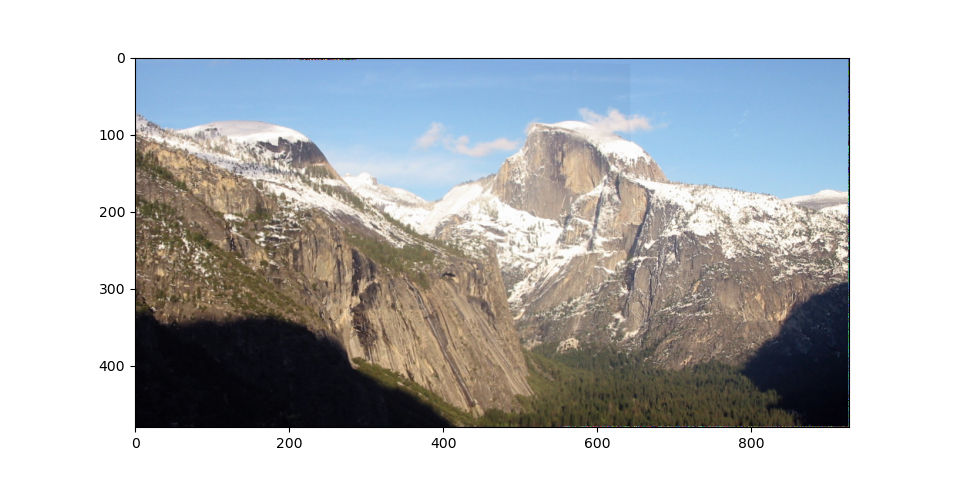
\includegraphics[width=\textwidth]{mosaico_yosemite_ransac_propio.png}
 		\caption{Mosaico de las imágenes de Yosemite utilizando la implementación propia de RANSAC.}
\end{figure}

\begin{figure}[H]
  \centering
      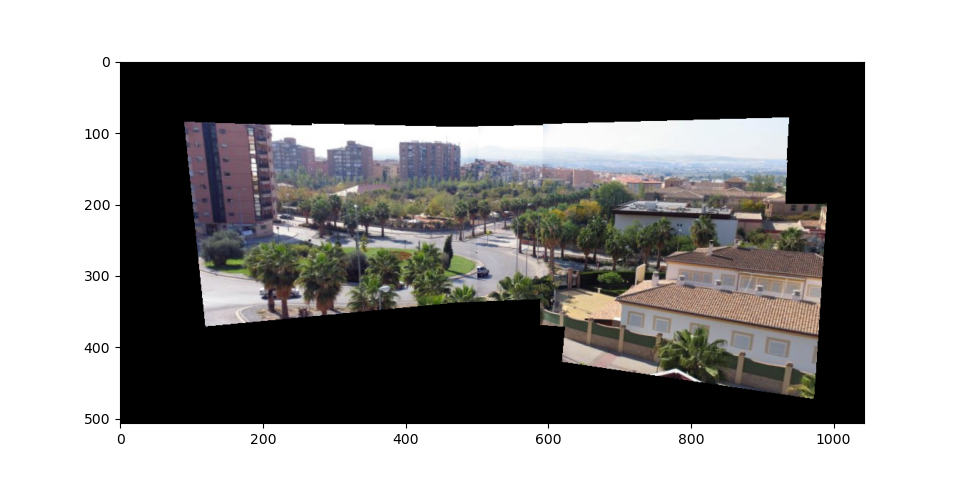
\includegraphics[width=\textwidth]{mosaico_etsiit_ransac_propio.png}
 		\caption{Mosaico de todas las imágenes de las vistas de la ETSIIT utilizando la implementación propia de RANSAC.}
\end{figure}


Vemos que a primera vista no hay diferencias entre la implementación propia y el uso de OpenCV, por lo que voy a mostrar una comparación directa de cada pareja de imágenes en una misma figura:

\begin{figure}[H]
  \centering
      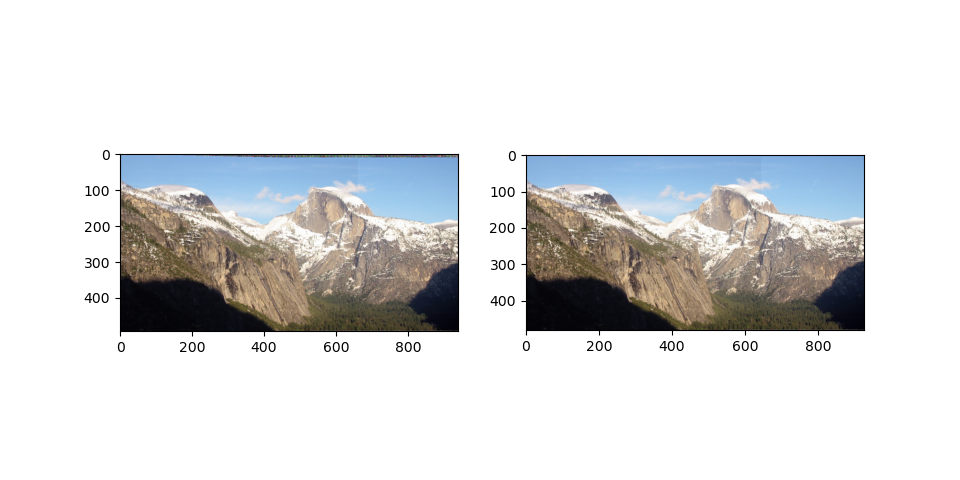
\includegraphics[width=\textwidth]{cmp_ransac_cv_propio.png}
 		\caption{Comparación entre mosaicos: A la izquierda utilizando OpenCV, a la derecha la implementación de RANSAC.}
\end{figure}

\begin{figure}[H]
  \centering
      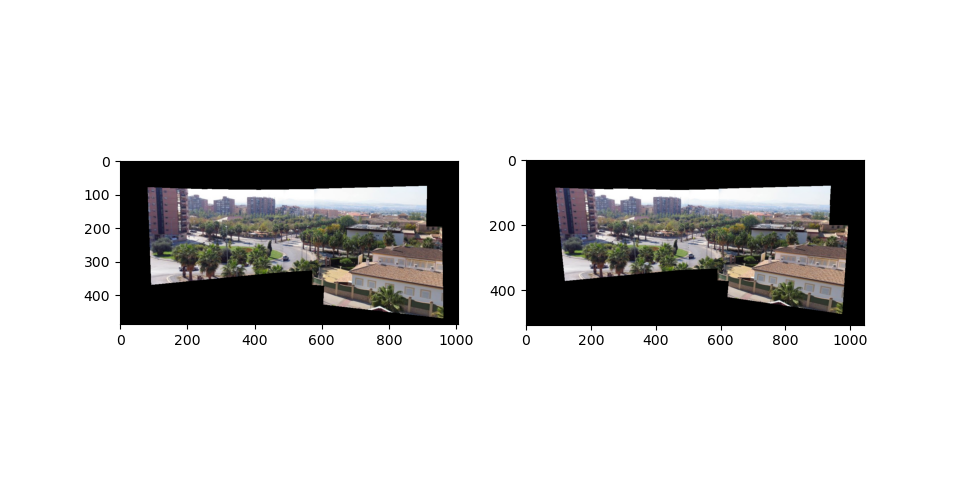
\includegraphics[width=\textwidth]{cmp_ransac_cv_propio_etsiit.png}
 		\caption{Comparación entre mosaicos: A la izquierda utilizando OpenCV, a la derecha la implementación de RANSAC.}
\end{figure}


En esta comparación, en especial el mosaico de la ETSIIT al ser más imágenes, si que percibimos una cierta diferencia en las imágenes de los extremos, que no coinciden exactamente los puntos en ambas soluciones. Esto sin embargo se trata de un error de redondeo a la hora de calcular la homografía, ya que OpenCV no conocemos como realiza la aproximación en profundidad y nuestra implementación propia está utilizando NumPy con números de coma flotante lo que añade cierto error de precisión en los cálculos.

Como conclusión, creo que mi aproximación del algoritmo es bastante buena, ya que es capaz de trabajar correctamente con todos los apartados antes desarrollados de la práctica sin tener que aplicar ninguna modificación (en la función para crear el panorama simplemente se ha cambiado la llamada a la función) y obtiene unos buenos resultados como he comentado.

\newpage

\section{Referencias, material y documentación usada}


\begin{thebibliography}{9}

	\bibitem{harris}

		Multi-Image Matching using Multi-Scale Oriented Patches --- Matthew Brown, Richard Szeliski y Simon Winder

		\url{http://matthewalunbrown.com/papers/cvpr05.pdf}

	\bibitem{kaze}

		KAZE Features --- Pablo F. Alcantarilla, Adrien Bartoli, and Andrew J. Davison (Enlace de Wayback Machine ya que el enlace original no funciona).

		\url{https://web.archive.org/web/20200125092345/http://www.robesafe.com/personal/pablo.alcantarilla/papers/Alcantarilla12eccv.pdf}

	\bibitem{akaze}

		Fast Explicit Diffusion for AcceleratedFeatures in Nonlinear Scale Spaces --- Pablo F. Alcantarilla, Jesús Nuevo and Adrien Bartoli (Enlace de Wayback Machine ya que el enlace original no funciona).

		\url{https://web.archive.org/web/20200114013631/http://www.robesafe.com/personal/pablo.alcantarilla/papers/Alcantarilla13bmvc.pdf}


	\bibitem{lowe}

		Distinctive Image Featuresfrom Scale-Invariant Keypoints --- David G. Lowe

		\url{https://www.cs.ubc.ca/~lowe/papers/ijcv04.pdf}

	\bibitem{ransac}

		Homography Estimation Using RANSAC --- Harshal Patil, Prof.S.S.Deshmukh

		\url{http://www.ijreat.org/Papers\%202013/Issue3/IJREATV1I3027.pdf}


	\bibitem{cornerCV}

		cornerEigenValsAndVecs --- Documentación oficial de OpenCV

		\url{https://docs.opencv.org/master/dd/d1a/group__imgproc__feature.html#ga4055896d9ef77dd3cacf2c5f60e13f1c}

	\bibitem{keypoint}

		Clase KeyPoint --- Documentación oficial de OpenCV

		\url{https://docs.opencv.org/master/d2/d29/classcv_1_1KeyPoint.html}

	\bibitem{cornerSubPix}

		cornerSubPix --- Documentación oficial de OpenCV

		\url{https://docs.opencv.org/master/dd/d1a/group__imgproc__feature.html#ga354e0d7c86d0d9da75de9b9701a9a87e}

	\bibitem{drawkKeypoints}

		drawKeypoints --- Documentación oficial de OpenCV

		\url{https://docs.opencv.org/master/d4/d5d/group__features2d__draw.html#ga5d2bafe8c1c45289bc3403a40fb88920}

	\bibitem{cAKAZE}

		Clase AKAZE --- Documentación oficial de OpenCV

		\url{https://docs.opencv.org/master/d8/d30/classcv_1_1AKAZE.html}

	\bibitem{detectCompute}

		detectAndCompute --- Documentación oficial de OpenCV

		\url{https://docs.opencv.org/master/d0/d13/classcv_1_1Feature2D.html#a8be0d1c20b08eb867184b8d74c15a677}

	\bibitem{BFMatcher}

		Clase BFMatcher --- Documentación oficial de OpenCV

		\url{https://docs.opencv.org/master/d3/da1/classcv_1_1BFMatcher.html}

	\bibitem{drawMatches}

		drawMatches --- Documentación oficial de OpenCV

		\url{https://docs.opencv.org/master/d4/d5d/group__features2d__draw.html#gad8f463ccaf0dc6f61083abd8717c261a}

	\bibitem{knnMatch}

		knnMatch --- Documentación oficial de OpenCV

		\url{https://docs.opencv.org/master/db/d39/classcv_1_1DescriptorMatcher.html#a378f35c9b1a5dfa4022839a45cdf0e89}

	\bibitem{match}

		match --- Documentación oficial de OpenCV

		\url{https://docs.opencv.org/master/db/d39/classcv_1_1DescriptorMatcher.html#a0f046f47b68ec7074391e1e85c750cba}

	\bibitem{findHomography}

		findHomography --- Documentación oficial de OpenCV

		\url{https://docs.opencv.org/master/d9/d0c/group__calib3d.html#ga4abc2ece9fab9398f2e560d53c8c9780}

	\bibitem{warpPerspective}

		warpPerspective --- Documentación oficial de OpenCV

		\url{https://docs.opencv.org/master/da/d54/group__imgproc__transform.html#gaf73673a7e8e18ec6963e3774e6a94b87}

\end{thebibliography}

\end{document}
